% Seminar Information Retrieval Philipp Schalcher
% Betreuer: Ruxandra Domenig
% Thema: Evaluierung der Retrieval-Leistung einer Search Engine am Beispiel einer privaten MP3-Sammlung

\documentclass[12pt,a4paper,ngerman]{report}
\setlength{\parindent}{0pt}
\usepackage[ngerman]{babel}
\usepackage[utf8]{inputenc}
\usepackage{a4wide}
\usepackage{graphicx}
\usepackage{url}
\usepackage[final]{listings}
\usepackage{color}
\usepackage{amsmath}
\author{Philipp Schalcher}
\title{Evaluierung der Retrieval-Leistung einer Search Engine am Beispiel einer privaten MP3-Sammlung}
\date{\today}

\begin{document}
%\maketitle
\begin{titlepage}
\begin{center}

\includegraphics[width=0.25\textwidth]{img/zhaw.png}\\[0.5cm]
\textsc{\Large Zürcher Hochschule für Angewandte Wissenschaften}\\[1.0cm]
\textsc{\Large Seminar Concurrent Programming}\\[1.5cm]

% Title
\hrulefill \\[0.5cm]
{\huge \bfseries File-Server in C anhand CRUDL}\\[0.4cm]
\hrulefill \\[0.5cm]
%Author und Betreuer
\begin{minipage}{0.4\textwidth}
\begin{flushleft}
\emph{Author:}\\
Philipp \textsc{Schalcher}
\end{flushleft}
\end{minipage}
\begin{minipage}{0.4\textwidth}
\begin{flushright}
\emph{Betreuer:}\\
Nicolas \textsc{Schottelius}
\end{flushright}
\end{minipage}

\vfill

%Datum
{\large \today}

\end{center}
\end{titlepage}
\pagenumbering{Roman}
\chapter*{Danksagung}
Ich möchte mich an dieser Stelle bei allen bedanken, die mich bei dieser Arbeit tatkräftig unterstützt haben.\\
\\
An erster Stelle bedanke ich mich bei Herr Nicolas Schottelius. Die spannende Arbeit zum Thema Concurrent Programming kam als Auftrag aus seiner Feder. Er motivierte uns, trotz mangelnder Kenntnisse in der C-Programmierung, die Aufgabe zu lösen. Dadurch erhielt ich die Chance, sehr viel zu lernen.\\
\\
An zweiter Stelle bedanke ich mich bei Herr Karl Brodowsky, unserem Dozenten im Bereich Systemsoftware. Seine C-Kenntnisse und Tipps haben ab und zu zur Lösungsfindung beigetragen. Wohl auch Dank seiner Unterstützung wurde das Programm lauffähig.\\
\\
Dann möchte ich Ramona Heiz, Doris Oberholzer und Yvonne Schalcher danken, welche mir als Lektorinnen dienten. Ohne sie wäre dieses Dokument wahrscheinlich unlesbar geworden. Geduldig arbeiteten sie sich durch das Dokument und halfen mir den Stoff verständlich und inhaltlich auszulegen. Danke für eure Geduld und Arbeit.
\tableofcontents
\begin{abstract}
Gleichzeitige Nutzung eines Serverprogramms  ist ein zentraler Aspekt des Servers. Daher muss das Programm sicherstellen, dass Ressourcen verfügbar oder gesperrt sind. In unserem Fall dreht sich alles um einen Dateiserver. Dieser soll sich um die Grundoperationen kümmern. Die Grundoperationen sind CREATE, READ, UPDATE, DELETE, LIST. Da jede Operation auf einer Datei von zwei Prozessen durchgeführt werden könnte, werden die Dateien gesperrt.\\
\\
Für jeden Client, der sich mit dem Server verbindet, wird ein neuer Prozess erstellt, der diesen Client bedient. Dadurch wird gewährleistet, dass mehrere Zugriffe gleichzeitig stattfinden können. Die Dateien selber werden in ein Shared-Memory gespeichert. So wird sichergestellt, dass die einzelnen Prozesse Zugriff auf die Dateien haben. Im Gegensatz zu Prozessen mit pthreads, muss bei fork ein Shared-Memory eingesetzt werden. fork teilt die Ressourcen nicht automatisch unter den Prozessen.\\
\\
Da nun einzelne Clients Operationen ausführen, wird die entsprechende Datei gesperrt, die gerade benutzt wird. Die trifft für LIST und CREATE nicht zu. Bei READ, UPDATE und DELETE wird der Semaphorwert aus der Datei ausgelesen und dementsprechend verwendet. So wird garantiert, dass kein Client eine Datei lesen kann, während ein anderer Client die Datei momentan aktualisiert.\\
\\
Verschiedene Herausforderungen sind während der Arbeit aufgetreten. Wie zum Beispiel beim zu kleinem Speicherbereich oder konzeptionellen Entscheidungen. Für zu kleinen Speicherbereich sei das Shared-Memory erwähnt. Dieses muss bei der Erstellung mit einer angemessenen Grösse bestückt werden, da sonst nicht genug Dateien erstellt werden können. Für den konzeptionellen Teil ist der Semaphor beispielgebend. In der ersten Version wurde ein einziger Semaphorwert genutzt. Allerdings kollidierte diese Lösung mit der Idee, dass verschiedene Dateien einander nicht beeinflussen. Auch wäre so ein globaler Lock entstanden, welcher von der Aufgabenstellung verboten war. Daher wurde ein Semaphorwert zu jeder Datei hinzugefügt. Das Problem löste sich und ein UPDATE auf eine Datei 1 hatte keinen Einfluss mehr auf ein READ der Datei 2.
\end{abstract}
\pagenumbering{arabic}
\setcounter{page}{1}
\chapter*{Einleitung}
Ein wichtiger Teil der Systemprogrammierung ist das Concurrent Programming. Dabei steht nicht die Parallelisierung im Vordergrund, sondern das Problem, von Zugriffen auf Ressourcen und die damit auftretenden Schwierigkeiten. Gleichzeitige Bearbeitungen von Ressourcen können, je nach ausgeführter Arbeit, zu schwerwiegenden Problemen führen. Wird zum Beispiel eine Datei gelöscht, obwohl die Datei momentan an einem anderen Ort geöffnet ist und das System dies nicht bemerkt, tritt ein Konflikt auf. Soll die Datei nun gelöscht werden und der Bearbeiter verliert den Zugriff, oder soll die Datei einfach nicht gelöscht werden, mit dem Vermerk, dass die Datei geöffnet ist?
\\
In dieser Arbeit soll nun ein Dateiserver in C programmiert werden, der genau solche Probleme abfangen soll. Dabei gilt, dass der Server nach dem Schema CRUDL funktionieren soll. CRUDL steht für:
\begin{itemize}
	\item CREATE
	\item READ
	\item UPDATE
	\item DELETE
	\item LIST
\end{itemize}
Je nach aufgerufenem Task, darf eine Datei nicht mehr zugreifbar sein.
\\
\\
Die Arbeit soll keine realen Dateien verarbeiten können. Das Ziel liegt in der Realisierung des CRUDL-Systems. Die Dateien selber werden in einem Shared-Memory gespeichert (nur die Dateinamen). Sobald der Server gestoppt wird, gehen die Dateien im Shared-Memory verloren.
\chapter{Anleitung}
Der Server kann über die Binary \textquotedblleft run\textquotedblright gestartet werden. Im Konsolenfenster werden Nachrichten zur Initialisierung ausgegeben. Sobald der Server gestartet ist, kann über das Binary \textquotedblleft test\textquotedblright ein Testclient gestartet werden. Über diesen können Befehle an den Server gesendet werden.
\section{Befehle}
Der Server erkennt folgende Befehle:
\begin{itemize}
	\item CREATE Dateiname Grösse
	\item READ Dateiname
	\item UPDATE Dateiname Grösse
	\item DELETE Dateiname
	\item LIST
\end{itemize}

\section{CREATE}
Syntax: CREATE \textit{Dateiname} \textit{Grösse} \\
CREATE erstellt eine neue Datei im Fileserver. Als Parameter wird der gewünschte Dateiname und die Grösse als Zahl mitgegeben. Falls die Datei schon vorhanden ist, gibt der Server ein \textquotedblleft FILEEXISTS\textquotedblright zurück. Andernfalls wird bei Erfolg die Nachricht \textquotedblleft FILECREATED\textquotedblright an den Client gesendet.\\
\\
Beispiel: CREATE meineErsteDatei 30
\section{READ}
Syntax: READ \textit{Dateiname}
READ liest den Inhalt einer Datei aus und sendet sie an den Client. Falls der Dateiname nicht existiert, wird die Nachricht \textquotedblleft NOSUCHFILE\textquotedblright zurückgegeben.\\
\\
Beispiel: READ meineErsteDatei
\section{UPDATE}
Syntax: UPDATE \textit{Dateiname} \textit{Grösse}\\
Mit UPDATE wird die vorhandene Datei geändert. Dabei wird die Grösse und der Inhalt verändert. Existiert der angegebene Dateiname nicht, wird die Nachricht \textquotedblleft NOSUCHFILE\textquotedblright zurückgegeben. Ist der Befehl erfolgreich, wird in einem zweiten Schritt der Inhalt verlangt.\\
\\
Beispiel: UPDATE meineErsteDatei 13
\section{DELETE}
Syntax: DELETE \textit{Dateiname}\\
Nach dem Aufruf von DELETE wird die ausgewählte Datei gelöscht. Dabei gibt der Befehl die Meldung \textquotedblleft NOSUCHFILE\textquotedblright zurück, falls kein Eintrag mit dem Dateinamen bekannt ist. Ansonsten erhält man die Nachricht \textquotedblleft DELETED\textquotedblright . \\
\\
Beispiel: DELETE meineErsteDatei
\section{LIST}
Syntax: LIST
LIST veranlasst den Server dazu, alle Dateien zu zählen und deren Namen an den Client zu senden.
\section{Beschränkung}
Durch den Einsatz der Semaphore ist der Server momentan auf maximal 10 gleichzeitige Read-Vorgänge eingeschränkt. Dies könnte mit grösserem Semaphor verändert werden. Da aber keine Angaben im Auftrag gemacht wurden, werde ich die Einstellung in diesem Zustand belassen.
\chapter{Ausgangslage}
Auf Wunsch des Dozenten in Concurrent Programming soll entweder ein Datei-Server oder ein Mehrbenutzereditor in C programmiert werden. Diese Arbeit behandelt die Aufgabe mit dem Datei-Server. Dabei muss der Server gewisse Bedingungen erfüllen. Diese wären:
\begin{itemize}
	\item Keine SEGV während des Betriebs.
	\item Jeder Client der verbindet, soll mit einem eigenen Prozess behandelt werden.
	\item Server muss nach CRUDL arbeiten.
	\item Das echte Dateisystem darf nicht genutzt werden.
	\item Dateien sind nur im Speicher vorhanden.
\end{itemize}

CRUDL bedeutet soviel wie CREATE, READ, UPDATE, DELETE und LIST. Diese 5 Befehle müssen vom Server umgesetzt werden. Der Fokus liegt dabei auf de  Zugriff von verschiedenen Prozessen auf Dateien. Gewisse Operationen wie z.Bsp. DELETE, müssen Dateien komplett sperren, damit diese während der Ausführung nicht von anderen Operationen besetzt werden können. Das heisst, während eines DELETE darf kein READ, UPDATE oder LIST durchgeführt werden. Innerhalb dieser Befehle gibt es mehrere Kombinationen solcher Sperrungen. Diese müssen abgefangen werden.
\section{Lösungsansatz}
Die Problematik besteht also aus drei Teilproblemen. Das erste Problem ist die Netzwerkverbindung und die darauf folgende Erstellung eines neuen Prozesses, der die Anfragen annimmt und verarbeitet. Als Lösung würde ich daher auf eine normale TCP/IP Verbindung setzen. Diese wird über Sockets gelöst. Sobald ein Client verbindet, wird per fork() ein neuer Prozess erstellt, der als Child-Prozess die Anfragen des Clients annimmt und bearbeitet. Innerhalb des Child-Prozesses müssen daher die Befehle abgefangen werden und die eigentlichen Aktionen ausgeführt werden.
\\
Als zweites Problem erachte ich die Speicherung der "Dateien". Hier würde ich so vorgehen, indem ich eine Struktur aufbaue, die für jede Datei ihren Dateinamen, ihre Grösse und den Inhalt speichert. Eine einzelne Struktur soll also eine Datei symbolisieren. Um mehrere Dateien speichern zu können, wird aus der Struktur ein Array erstellt. Leider begrenzt ein Array die Anzahl der zu verarbeitenden Dateien. Allerdings könnte dies gleichgesetzt werden mit dem Plattenspeicher, der irgendwann auch voll ist.
\\
Als drittes Problem ist die Sperrung der Dateien ein zentraler Punkt. Da für den Server keine globalen Sperren genutzt werden dürfen, würde ich Semaphore einsetzen, welche die einzelnen Codeteile sperren und so von Prozessen nicht gleichzeitig ausgeführt werden können. Der Semaphor an sich muss aber mehr als ein "Ticket" vergeben können, da zum Beispiel READ mehrfach ausgeführt werden darf. Jedoch muss ein DELETE den kompletten Semaphor besetzen, damit keine anderen Operationen durchgeführt werden können.
Auch hier gilt wieder, dass mit der Semaphorengrösse auch die Anzahl Clients beschränkt wird. So können bei einem Semaphor mit 10 Tickets maximal 10 Clients gleichzeitig einen READ durchführen. Auch wenn 20 Clients verbunden wären, so würden doch immer nur 10 bedient werden.
\chapter{Realisierung}
In diesem Kapitel werde ich auf die Realisierung eingehen. Ein kurzer Abschnitt handelt von meiner Vorgehensweise und wie ich den Server aufgebaut habe. Schwerpunkt wird allerdings auf den Bereich \textquotedblleft Schwierigkeiten\textquotedblright und \textquotedblleft Testing\textquotedblright gelegt.
\section{Implementation}
Der ganze Server ist in einem C-Sourcefile zu finden. Der Aufbau ist relativ einfach:
\begin{itemize}
	\item Includes der Bibliotheken
	\item Globale Variablen definieren
	\item Funktionen definieren
	\item Main-Funktion Definition
		\begin{itemize}
		\item Erstellung des Signal-Handlers
		\item Erstellung des Shared-Memory
		\item Erstellung des Semaphors
		\item Aufbau des Netzwerkteils
		\item Abfangen von Verbindungsanfragen und Prozesserstellung
			\begin{itemize}
			\item Abfangen des LIST-Befehls
			\item Abfangen des CREATE-Befehls
			\item Abfangen des READ-Befehls
			\item Abfangen des UPDATE-Befehls
			\item Abfangen des DELETE-Befehls
			\end{itemize}
		\end{itemize}
\end{itemize}
Die komplette Logik ist im Bereich der Befehlsabfragen zu finden. Die Dateien werden in einer definierten Struktur gespeichert, welche als Array auf das Shared-Memory gelegt wird. Sobald ein freier Platz oder eine bestimmte Datei gesucht werden muss, durchläuft eine Schlaufe das Array, bis die Länge des Strings im Namen gleich 0 ist. So wissen wir, dass wir die letzte Position erreicht haben. Wie die Befehle genau implementiert sind, wird in den folgenden Abschnitten erklärt.
\subsection{Implementation LIST}
Für den Befehl List, wird das Array durchgelaufen und die Anzahl gefundener Dateien gezählt. Da auch Einträge mit Namen \textquotedblleft EMPTY\textquotedblright vorkommen können (mehr dazu im Kapitel \textquotedblleft Implementation DELETE\textquotedblright), werden diese ignoriert. Die korrekten Dateinamen werden an einen vorhandenen String angehängt. Ist die letzte Position im Array erreicht, wird die Nachricht generiert und an den Client gesendet. Danach steht der Server wieder für die nächste Eingabe zur Verfügung.
\subsection{Implementation CREATE}
Das Array wird wieder durchgegangen bis das Ende erreicht ist (wieder über die Längenprüfung von Name) oder ein Eintrag mit \textquotedblleft EMPTY\textquotedblright gefunden wird. Ist der vorgegebene Dateiname schon vorhanden, bricht der Vorgang ab. Ansonsten wird der Name, die Grösse sowie der Semaphorwert gesetzt und der Client wird nach dem Inhalt gefragt. Der Client muss den Inhalt eingeben, welcher dann im Feld Content gespeichert wird.
\subsection{Implementation READ}
Das Array wird nach dem angegebenen Namen durchsucht. Wird kein Eintrag gefunden, erhält man ein \textquotedblleft NOSUCHFILE\textquotedblright . Ansonsten holt sich der Prozess ein Semaphorticket und liest den Inhalt. Der Inhalt wird dann an den Client gesendet. Zum Abschluss gibt der Prozess das Semaphorticket wieder zurück. Sind alle Tickets verbraucht, wartet der Prozess bis eines frei wird.
\subsection{Implementation UPDATE}
Der erste Teil ist gleich wie im READ-Bereich. Ist das spezifische File gefunden, werden zuerst alle Semaphortickets reserviert, dann die Grösse und der Inhalt auf Leer geändert. Der Server fragt danach wieder den Client an, um den Inhalt zu erhalten. Sobald der Client den Inhalt generiert hat und zurückgegeben wurde, speichert der Server die Werte im Feld Content. Danach werden die Semaphortickets zurückgegeben. Solange UPDATE aktiv ist, kann kein READ, DELETE oder UPDATE durchgeführt werden.
\subsection{Implementation DELETE}
Falls bei einem Löschvorgang der Name auf NULL gesetzt wird, erhält das Array einen zweiten Punkt, wo die Stringlänge ebenfalls gleich 0 ist. Daraus folgt, dass das Array nicht mehr komplett durchgelaufen werden kann. Daher wird der Name nur auf \textquotedblleft EMPTY\textquotedblright gesetzt. So ist garantiert, dass das Array immer komplett durchgelaufen werden kann. Die restlichen Einträge werden auf NULL, 0 oder leer gesetzt.
\subsection{Implementation Semaphor}
Im Array enthält jeder Eintrag eine Variable semval. Diese beinhaltet die maximalen Tickets für eine Datei. In den einzelnen Befehlsbereichen wird bei der Ausführung der Wert ausgelesen und per semctl in den Semaphor geladen. Danach holt sich der Prozess ein oder alle Tickets per semop. Sobald der kritische Bereich ausgeführt worden ist, wird das reservierte Ticket frei gegeben.
\begin{figure}[h!]
\centering
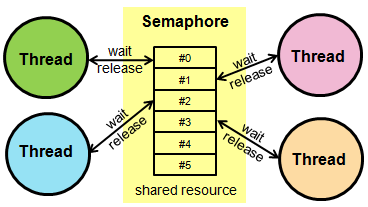
\includegraphics[width=10cm]{img/semaphore.png}
\caption{Semaphor sperrt Ressource für Threads\protect\footnotemark}
\end{figure}
\footnotetext{Quelle: \url{http://www.mbed.org}}
\section{Schwierigkeiten}
In diesem Abschnitt möchte ich auf einige Probleme eingehen, die bei der Erstellung des Servers aufgetreten sind. Im Anschluss zu den jeweiligen Problemen wird meine Lösung angegeben.
\subsection{Struktur Datei}
In der Struktur Datei werden die Informationen zu den Dateien gespeichert. Hier gab es zwei grosse Entscheidungen bei der Implementation. Das erste Problem bestand in der Definition von der Variable Name und Content. Sind diese als undefinierte Arrays von Chars deklariert, zeigt der nächste Eintrag im Strukturarray auf den gleichen Speicher, wie der vordere. So entstand das Problem, dass ein zweiter Eintrag den Namen des ersten Eintrages änderte. Dies ging so weiter für jeden folgenden Eintrag in der Struktur.\\
\\
Das zweite Problem lag beim Durchsuchen. Der Name im Array wurde als Referenz genutzt. Der Durchlauf per Schlaufe lief mit der Prüfung auf NULL aber nur schlecht durch. Auch funktionierte er teilweise nicht, so dass das Programm hängen blieb und nicht mehr reagieren konnte.
\subsubsection{Lösung}
Problem 1 kam aus der Eigenschaft des undefinierten Arrays. Der Speicher der Namensvariable zeigt für alle Einträge im Strukturarray auf die gleiche Adresse. So entstand die Eigenschaft, dass jeder weitere Eintrag den Namen auf die vorhergehenden Einträge vererbte. Die Lösung war, dass der Name nicht mehr eine undefinierte Länge besitzt, sondern das Char-Array von Beginn an auf eine bestimmte Grösse definiert wurde.\\
\\
Problem 2 liess den Server an einer bestimmten Stelle einfrieren. Dieser Effekt war aber nicht voraussagbar, da er nur sporadisch auftrat. Die Änderung der while-Schleife auf die Prüfung der Stringlänge behob dieses Problem. 
\subsection{Generierung Messages}
Es trat das Problem auf, dass die Rückmeldungen (besonders bei der Funktion LIST) nicht korrekt in die Stringvariable geschrieben wurden. Im schlimmsten Fall blieb der Server an einem bestimmten Punkt bei der Ausführung stecken.
\subsubsection{Lösung}
Zwei verschiedene Lösungen hatten sich bei der Implementierung angeboten. Da der Inhalt meistens mit strcpy oder strcat gebaut wird, lag das Problem bei der Vorbereitung des Speichers. Bei der ersten Variante setzte ich für die Speicherreservierung ein malloc() ein. Allerdings funktionierte diese Lösung nur begrenzt. Die Nachricht wurde, aufgrund der Grösse bei mehreren Dateien, nicht mehr anzeigbar. Die letzten Dateien wurden nicht mehr in den String eingefügt.Die Anpassung der Grösse bei malloc() hat leider nicht zum gewünschten Erfolg geführt. Daher stellte ich die Nachrichtenvariable auf eine feste Grösse um. Der Speicher wurde so reserviert und alle Dateien konnten angezeigt werden. Je nach Grösse der Dateiliste kann auch hier dieses Problem wieder auftauchen.
\newpage
\subsection{Semaphore und Dateien}
Da die Semaphorwerte in der Struktur der Datei gespeichert werden und für jede Operation ausgelesen werden müssen, wird auch immer der Befehl semctl() ausgeführt. Es entstand das Problem, dass bei mehrfachen Zugriffen die Werte immer wieder zurückgesetzt wurden. So hatte der Semaphor den Wert 10 beim Start, nach dem ersten semop() des UPDATES wurde er 0. Ein READ-Befehl setzte hingegen den Wert des Semaphors wieder auf 10. Der Semaphor sperrte einerseits den Zugriff, wurde aber andererseits automatisch erhöht und die Sperre dadurch umgangen.
\subsubsection{Lösung}
Der Wert aus dem Semaphor soll wieder zurück in die Datei geschrieben werden. Der Wert der Variable ändert sich während der Laufzeit und passt sich an. Werden 10 Plätze reserviert, so steht in der Variable innerhalb der Struktur danach der Wert 0. Ein zweiter Prozess liesst diese vor semctl() aus und erhält so den aktuellen Semaphorwert. Einzelne Dateien werden so gesperrt, ohne dass andere Dateien beeinträchtigt sind.
\section{Testing}
Das Testing wurde während des Entwicklungsprozesses in den Fokus gelegt. Die Tests wurden manuell durchgeführt mit dem Binary test. Das Binary wechselt ausschliesslich zwischen read() und write() per TCP. Der Server musste sich dementsprechend anpassen.
\subsection{Test 1: Netzwerk}
Der erste Test kümmerte sich nur um die Verbindung zum Server. Er war erfolgreich, sobald ein Client (test) verbinden konnte, was reibungslos klappte.
\subsection{Test 2: Fork}
Der zweite Test überprüfte das Handling von mehreren Clients. Nachdem der fork() in den Server eingebaut wurde, testete ich mit 4 Clients einen gleichzeitigen Zugriff. Dies funktionierte und die Prozesse des Servers kümmerten sich um die Clients.
\subsection{Test 3: Befehlsabfrage}
Durch strtok wird der übermittelte String aufgeteilt. So konnte ich vergleichen, welchen Befehl der User abgesetzt hat. Der Test lief darauf hinaus, dass bei der erfolgreichen Erkennung eine Nachricht ausgegeben wurde.
\subsection{Test 4: Dateioperationen}
Nach der Implementation der Befehle testete ich die einzelnen Befehle mit dem Client. Dabei galt, dass mehrere Dateien erstellt (maximal 10 gestestet), gelesen, aktualisiert und gelöscht werden mussten. Dieser Test brauchte einige Zeit, da immer wieder kleine Änderungen am Code vorgenommen werden mussten. Daher ging ich so vor, jeden Befehl einzeln zu implementieren und zu testen. Erst als die Befehle funktionierten, ging ich zum nächsten über. Als Letztes kümmerte ich mich um LIST. So konnte ich sicherstellen, dass die Befehle korrekt arbeiten.
\subsection{Test 5: Shared Memory}
Für diesen Test benutzte ich zwei Clients, die sich mit dem Server verbanden. Danach erstellte ich einige Dateien. Nun wechselte ich in den zweiten Client und verband mit dem Server. Mit dem Befehl LIST musste ich nun als erfolgreiches Ergebnis die Dateinamen erhalten. 
\subsection{Test 6: Semaphor}
Als letzten Test betrachtete ich die Sperrung der Dateien. Auch hier verband ich wieder zwei Clients mit dem Server und erstellte einige Dateien. Nun musste Client 1 ein UPDATE auf eine Datei ausführen. Da der Client nach diesem Befehl den Inhalt verlangt, kann ich dadurch eine Datei auf unbestimmte Zeit sperren. Während Client 1 die Eingabe abwartete, versuchte ich ein READ im Client 2 auf die gleiche Datei auszuführen. Nach meiner Idee sollte nun beim READ nichts passieren, bis in Client 1 der Inhalt eingefügt wurde. Da ich nur mit UPDATE eine Sperre bauen konnte, habe ich die Schlussfolgerungen aus den Tests analog auf die restlichen Befehle übertragen.
\chapter{Fazit}
Die Aufteilung des Projektes in einzelne Teilprobleme war eine gute Entscheidung. Dadurch konnte ich mich auf kleinere Teile des Servers konzentrieren. Ebenfalls praktisch hat sich die Entscheidung für fork(), Shared-Memory und Semaphore herausgestellt. Anstelle für die Prozessgenerierung pthreads zu benutzen, fiel mir der Gebrauch von fork() wesentlich einfacher. Allerdings hätte mit pthread kein Shared-Memory benutzt werden müssen, weil Speicher zwischen pthreads von alleine schon geteilt wird. Somit musste ich für meinen fork()-Ansatz ein Shared-Memory aufbauen. Dieses verwende ich ausschliesslich für die Speicherung der Dateien. Der Aufbau des Memory ging relativ einfach von der Hand.\\
\\
Mehr Arbeit hat die Befehlsabfrage abverlangt. Da mir Befehle wie strtok nicht bekannt waren, brauchte es viel Aufwand im Bereich der Informationssuche. Auch die aufgetretenen Probleme lagen meistens daran, dass mir die Erfahrung in der C-Programmierung fehlt. Konzeptionell hatte sich aber mein Vorgehen als erfolgreich gezeigt. \\
\\
Als grosse Herausforderung hat sich der Einbau der Semaphoren herausgestellt. Mein erster Ansatz, mit einem Semaphorwert stellte sich als suboptimal heraus. So hätten sich zwei verschiedene Dateien gesperrt, auch wenn das nicht nötig gewesen wäre. Daher änderte ich die Wertzuweisung so, dass jede Datei eine eigene Variable enthält, welche den Semaphorwert speichert. Aus diesem Grund muss auch der Semaphorwert nach jeder Operation wieder in die Variable geschrieben werden. Ebenfalls muss der Wert vor jeder Operation wieder aus der Variable in den Semaphorteil geladen werden. Diese Lösung mag umständlich sein, aber ist für meine Kenntnisse die zuverlässigste.\\
\\
Das Projekt war sehr interessant. Es gab mir die Möglichkeit, viel über die Programmierung mit C zu lernen. Die Aufgabenstellung mit dem File-Server war gut vorstellbar und brachte meiner Meinung nach den Vorteil, dass die Vorgaben zum Concurrent Programming klar verständlich waren. Ein gutes Beispiel oder eine bildliche Darstellung hilft meistens mehr, einen Auftrag zu verstehen, als diesen nur in theoretischer Form zu erhalten.
\chapter*{Glossar}
\textbf{Semaphor}\\
Ist eine Struktur, die dazu dient, Ressourcen während der Ausführung zu Sperren. Sie funktioniert nach dem Schema, dass ein Ticket für eine Operation geholt werden muss, und am Ende zurückgegeben wird. Falls kein Ticket vorhanden ist, wird keine Operation ausgeführt.\\
\\
\textbf{Shared-Memory}\\
Ein Teil des RAM wird für die Datenspeicherung reserviert. Auf diesen Speicherbereich hat jeder Prozess Zugriff. Shared-Memory ist ein wichtiger Teil in der Interprozesskommunikation.\\
\\
\textbf{SEGV}\\
Steht für Segmentation Fault oder Segmentation Violation. Es handelt sich hierbei um einen Fehler während der Ausführung, wenn zum Beispiel auf einen Speicher zugegriffen werden will, welcher gesperrt oder nicht verfügbar ist. \\
\\
\textbf{Sockets}\\
Sockets sind dazu da, dass Computer miteinander Daten austauschen und kommunizieren können. \\
\\
\textbf{fork / pthread}\\
Stehen für zwei verschiedene Methoden, wie aus einem Programm ein weiterer Prozess erzeugt werden kann. Der neu erzeugte Prozess wird als Kindprozess bezeichnet, während der Erzeuger als Vaterprozess betitelt wird.\\
\\
\textbf{String}\\
Ist eine Variable, die ausschliesslich Text beinhaltet. In C existieren diese nicht wie bei Java. Daher werden sie als Array von einzelnen Zeichen (Char) aufgebaut.\\
\\
\textbf{Array}\\
Ein Array ist eine Ansammlung von Werten des gleichen Types. Wichtig ist dabei, dass mehrere Werte in einem Array gespeichert werden können. Diese Arrays können dann durchlaufen werden, um einzelne Einträge zu erhalten.
\bibliography{document}
\bibliographystyle{plain}
\nocite{socketserver}
\nocite{fork1}
\nocite{fork2}
\nocite{socketclient}
\nocite{stcmp}
\nocite{substring}
\nocite{gitbk}
\nocite{semctl}
\nocite{unix_environment}
\end{document}